\chapter{Differential Equations}

In the last chapter we said that any equation involving derivatives of a function is called a differential equation.  In
this chapter we explore this idea further and look at some mathematical models that take the form of differential equations.  Change
is a concept that we are familiar with.  When we are imagining what something we are familiar with today will
be like in the future we can be pretty certain that it will be different.  Differential equations can arise when
we formulate mathematical models.  We can develop our understanding of this process by considering the mathematical
models of some physical phenomena. 

\section{Population Growth}
One model of population growth arises from the assumption that the rate at which the population grows is proportional to the size of the population.
\ Let $N$ be the size of the population at time
$t$ then the rate of change of population with respect to time is $\frac{d N}{d t}\text{.}$  So the model can be expressed as a differential equation
\begin{equation*}\frac{d N}{d t} =k N
\end{equation*}

where $k$ is the constant of proportionality. 

To make any sense of this model we need to explore the range of values
of $N$ and $k$.  $N$ cannot be zero (otherwise there would be nothing to change).  We assume that $N$ is a function of $t$ and that $N (t) >0$.  Similarly for us to have population ``growth''\  $k >0$
\begin{equation*} \therefore \frac{d N (t)}{d t} >0
\end{equation*}

We have already shown the properties of the exponential function.  The
general exponential function is
\begin{equation*}N (t) =N_{0} e^{k t}
\end{equation*}

Let $N (t)$ be $N_{0}$ when $t =0$.  i.e. $N (0) =N_{0}\text{.}$  $N_{0}$ is called the \emph{initial value} of $N (t)$. 

Now
\begin{align*}\frac{d N (t)}{d t} &    = N_{0} e^{k t} \times k \\
 &    = k N (t)\end{align*}

Thus we have shown that $N (t) =N_{0} e^{k t}$ is a solution of the differential equation $\frac{d N (t)}{d t} =k N (t)$ 

This solution arises because we are familiar with the behaviour of the exponential function.  Our
ability to ``guess''\ the answer is limited so the subject of differential equations involves developing
techniques to handle physical situations that are more and more realistic and more and more complex.  The answer
to this problem came so simply to us we have to wonder if there are other equations for $N (t)$ that give the same answer. 

\section{The Order of a Differential Equation}
The differential equation $\frac{d N (t)}{d t} =k N (t)$ is referred to as a first order differential equation because the order of the highest derivative is \emph{one}.
\ Here is an example of a second order differential equation
\begin{equation*}m \frac{d^{2} x}{d t^{2}} = -k x
\end{equation*}

$\frac{d^{2} x}{d t^{2}}$ is a second derivative.  This is the differential equation that arises from Hooke's Law.
\ This subject will be developed further in later courses. 

\section{The Solution of a Differential Equation}
When you are asked to ``solve''\ a differential equation you are expected to find all possible
solutions of the differential equation.  In chapter 4 we met a range of simple differential equations and showed
how to express all possible solutions. 

\subsubsection{Example 1}
Find all possible solutions of the differential equation $\frac{d y}{d x} =2 x\text{.}$  This differential equation could also be expressed as $y^{ \prime } =2 x\text{.}$ 

By antidifferentiating we obtain
\begin{equation*}y =x^{2} +C
\end{equation*}

Where $C$ is the constant of integration.  This is an arbitrary constant and gives us a family
of functions all of which are solutions of the differential equation $y^{ \prime } =2 x$.  This family of solutions is often referred to as the \emph{general solution}.


In a physical situation we are often provided with additional information and this will allow us to find a \emph{particular
solution}.  This is easy to visualise when considering $y^{ \prime } =2 x\text{.}$  The general solution is $y =x^{2} +C$ and if you are also told that the curve passes through $\left (2 ,6\right )$ you can use this information to evaluate $C\text{.}$
\begin{align*}6 &    = 2^{2} +C \\
C &    = 2\end{align*}

So the particular solution is $y =x^{2} +2$.  To appreciate the concept of this particular solution you only need to use Omnigraph to
draw $y =x^{2} +C$ for various values of $C$. 

\subsection{Initial-Value Problems}
In a physical problem when you are given the conditions for the particular solution in the form $y (t_{0}) =y_{0}$ where $t_{0}$ is the initial value of $t$ and $y_{0}$ is the initial value of $y (t)$, the point $\left (t_{0} ,y_{0}\right )$ is called an \emph{initial condition} and the
problem of finding the particular solution given the differential equation is referred to as an \emph{initial-value problem}. 

\subsubsection{Example 2}
For the differential equation $y^{ \prime } = -y^{2}$ 

(a) Verify that $y =\frac{1}{t +C}$ is the general solution 

(b) Find the solution of the initial-value problem $y^{ \prime } = -y^{2}$ and $y \left (0\right ) =0.5$ 

\textbf{Solution} 

(a) Given $y =\frac{1}{t +C} =\left (t +C\right )^{ -1}$
\begin{align*}y^{ \prime } &    =  -\left (t +C\right )^{ -2} \\
 &    = \frac{ -1}{\left (t +C\right )^{2}} \\
 &    =  -\genfrac{(}{)}{}{}{1}{t +C}^{2} = -y^{2}\end{align*}

So $y =\frac{1}{t +C}$ is the general solution of $y^{ \prime } = -y^{2}$ 

(b) Substitute $\left (0 ,0.5\right )$ in $y =\frac{1}{t +C}$
\begin{align*}0.5 &    = \frac{1}{0 +C} \\
\frac{1}{2} &    = \frac{1}{C} \\
C &    = 2\end{align*}

The particular solution is $y =\frac{1}{t +2}$ 

\subsection{Exercises 7.3}
\begin{enumerate}
\item Solve the following differential equations and use the given conditions to find the particular solution 


\begin{enumerate}
\item $\frac{d y}{d t} =e^{t} +2 t\text{\quad \quad }y (0) =2$ 

\item $\frac{d y}{d x} =\sin  2 x +\cos  2 x\text{\quad \quad }y (0) =0$ 

\item $t \frac{d y}{d t} =1 -t^{2}\text{\quad \quad }y \left (0\right ) =2$ 

\item $x^{2} \frac{d P}{d x} =2 +x\text{\quad \quad }P (1) =2$ \end{enumerate}


\item Show that $y =x +\frac{1}{x}$ is a solution of the differential equation $x y^{ \prime } +y =2 x$ 

\item Verify that $y =\sin  x \cos  x -\cos  x$ is a solution of the initial-value problem
\begin{equation*}y^{ \prime } +\left (\tan  x\right ) y =\cos ^{2} x\text{\  \  \  \  \  \  \  \  }y (0) = -1
\end{equation*} \\\relax on the interval $\frac{ -\pi }{2} <x <\frac{\pi }{2}\text{.}$ 

\item Which of the following functions are solutions of the differential
equation $y^{ \prime  \prime } +y =\sin  x$ \\\relax (a)  $y =\sin  x\text{\quad \quad }$(b)  $y =\cos  x\text{\quad \quad }$(c)  $y =\frac{1}{2} x \sin  x\text{\quad \quad }$(d)  $y = -\frac{1}{2} x \cos  x$ 

\item A mass falling to earth with a constant acceleration of $9.8 \mathrm{m}/\mathrm{s}^{2}$ satisfies the differential equation
\begin{equation*}\frac{d v}{d t} =9.8
\end{equation*} \\\relax where $v$ is the velocity at time $t$.  Find an expression for $v$ if 


\begin{enumerate}
\item The mass is dropped from a stationary position. 

\item The
mass is fired towards earth with an initial velocity of $100 \mathrm{m}/\mbox{s}\text{.}$ \end{enumerate}


\item The angular velocity
$\omega $ of a flywheel under constant braking torque of $N$ is given by the differential equation
\begin{equation*}I \frac{d \omega }{d t} +N =0.
\end{equation*}where $I$ is the moment of inertia ($I$ is a constant) 


\begin{enumerate}
\item Find $\omega $\ in terms of $t$ given that $\omega  =\omega _{0}$ when $t =0$. 

\item Calculate the time taken to bring the flywheel to rest from an initial
speed of $60 \pi  rad/\mbox{s}$ given that the moment of inertia is $100 kg \centerdot \mathrm{m}^{2}$ under a braking torque of $40 \mathrm{N} \centerdot \mbox{m}\text{.}$ \end{enumerate}
\end{enumerate}


\section{Separable Equations}
In some special cases we can find explicit solutions of differential equations. One type of equation can be written in the form
\begin{equation*}\frac{d y}{d x} =\frac{f (x)}{g (y)}
\end{equation*}

Expressed in this form we simply have to recognise that $f (x)$ is a function without any $y$'s in it and $g (y)$ is a function without any $x$'s in it. 

To solve $\frac{d y}{d x} =\frac{f (x)}{g (y)}$ we rewrite the equation as
\begin{equation*}g (y) d y =f (x) d x
\end{equation*}Then we integrate both sides
\begin{equation*}\int g (y) d y =\int f (x) d x
\end{equation*}This procedure can be verified by differentiating both sides with respect to $x$
\begin{equation*}\frac{d}{d x} \int g (y) d y =\frac{d}{d x} \int f (x) d x
\end{equation*}By the chain rule the left hand side becomes
\begin{equation*}\frac{d}{d y} \int g (y) d y \times \frac{d y}{d x}
\end{equation*}So
\begin{align*}\frac{d}{d y} \int g (y) d y \times \frac{d y}{d x} &    = \frac{d}{d x} \int f (x) d x \\
g (y) \times \frac{d y}{d x} &    = f (x) \\
\text{or\  \  \ }\frac{d y}{d x} &    = \frac{f (x)}{g (y)}\end{align*}

\subsubsection{Example 1}
Solve $\frac{d y}{d x} =\frac{x^{2}}{y^{2}}$
\begin{align*}y^{2} d y &    = x^{2} d x \\
\int y^{2} d y &    = \int x^{2} d x \\
\frac{y^{3}}{3} &    = \frac{x^{3}}{3} +C \\
y^{3} &    = x^{3} +3 C \\
 &    = x^{3} +C_{1}\end{align*}Where $C_{1}$ is a new arbitrary constant
\begin{equation*}y =\sqrt[{3}]{x^{3} +C_{1}}
\end{equation*}Find $C_{1}$ given $y (0) =2$
\begin{align*}2 &    = \sqrt[{3}]{0^{3} +C_{1}} \\
C_{1} &    = 8 \\
y &    = \sqrt[{3}]{x^{3} +8}\end{align*}

\subsubsection{Example 2}
Solve $y^{ \prime } =3 x^{2} y$ 

\textbf{Solution} 

First write $y^{ \prime } =\frac{d y}{d x}$ 

\begin{equation*}\frac{d y}{d x} =3 x^{2} y
\end{equation*}Separate the variables
\begin{equation*}\frac{1}{y} d y =3 x^{2} d x
\end{equation*}Integrate
\begin{align}\int \frac{1}{y} d y &    = \int 3 x^{2} d x \nonumber  \\
\ln  \left \vert y\right \vert  &    = x^{3} +C \tag{1}\end{align}We usually write this by writing in exponential form
\begin{align*}\left \vert y\right \vert  &    = e^{x^{3} +C} \\
 &    = e^{x^{3}} e^{C} \\
y &    =  \pm e^{C} e^{x^{3}}\end{align*}And write $A = \pm e^{C}$ where the value of $A$ is used that satisfies the particular problem
\begin{equation}y =A e^{x^{3}}\tag{2}
\end{equation}

In practice we usually jump from line (1) to line (2) and leave out the intermediate steps. 

\subsection{Exercises 7.4}
\begin{enumerate}
\item Solve the following differential equations 


\begin{enumerate}
\item $y \frac{d y}{d x} =x\text{\quad \quad }$given $y =4$ when $x =0$ 

\item $\frac{1}{t} \frac{d v}{d t} =2\text{\quad \quad }$given $v =2$ when $t =1$ 

\item $e^{x} \frac{d y}{d x} +2 =0\text{\quad \quad }$given $y =5$ when $x =0$ 

\item $\left (x +2\right ) \frac{d y}{d x} =y +3\text{\quad \quad }$given $y =0$ when $x =0$ 

\item $\frac{d i}{d t} +i =1\text{\quad \quad }$given $i =10$ when $t =0$ 

\item $\frac{d y}{d x} -2 x =0\text{\quad \quad }y (0) =2$ \end{enumerate}


\item The rate at which the atoms
of a radioactive substance split up is given by $\frac{d N}{d t} = -\lambda  N\text{,}$ where $N$ is the number of atoms present after $t$ seconds and $\lambda $\ is a constant. 


\begin{enumerate}
\item Show that $N =N_{0} e^{ -\lambda  t}$ where $N_{0}$ is the number of atoms present initially (i.e. when $t =0$). 

\item Find the time in years for half of the atoms of a given mass of
radium to disintegrate if $\lambda  =1.37 \times 10^{ -11}$\ for radium. \end{enumerate}


\item A
body falling in a medium where the resistance is proportional to the velocity $v$ at time $t$ obeys the differential equation $\frac{d v}{d t} =10 -0.2 v$ 


\begin{enumerate}
\item If the body falls from rest find $v$ in terms of $t$ and show that as $t \rightarrow \infty $ the velocity approaches $50 \mathrm{m}/\mbox{s}$. 

\item How long would it take for the body to reach a velocity of $25 \mathrm{m}/\mbox{s}$? \end{enumerate}


\item On a hot summer's day a
bottle of beer is placed in a fridge set at $4 \mbox{{\ensuremath{{}^\circ}}C}$.  The rate of change of the bottle's temperature
$\theta  \mbox{{\ensuremath{{}^\circ}}C}$ after $t$ minutes is given by Newton's Law of Cooling, $\frac{d \theta }{d t} = -k \left (\theta  -4\right )$ where $k$ is a constant that is specific to the beer. 


\begin{enumerate}
\item Find $\theta $ in terms of $t$.  If the initial temperature ($t =0$)\ of the bottle of beer was $22 \mbox{{\ensuremath{{}^\circ}}C}$ and it took $10 \mbox{min}$ to cool to $20 \mbox{{\ensuremath{{}^\circ}}C}\text{,}$ find the value of $k$, and the particular solution. 

\item How long would it take the bottle to
reach the ideal drinking temperature of $8 \mbox{{\ensuremath{{}^\circ}}C}$? \end{enumerate}


\item Brine
containing $2$ grams of salt per litre flows into a tank initially filled with $50$ litres of water containing $10$ grams of salt.  The brine enters the tank at $5$ litres/$\mbox{min}$, the concentration is kept constant by stirring and the mixture flows out through a tap at
the same rate so that the tank at all times continues to contain $50\,$L of mixture.  Let there be $Q$ grams of salt in the tank after $t$ minutes. 


\begin{enumerate}
\item Show that $\frac{d Q}{d t} =10 -\frac{Q}{10}$ 

\item Solve this differential equation to obtain an expression for $Q$ in terms of $t$. 

\item How much salt is in the tank after $10$ minutes? 

\item Sketch the graph of $Q$ against $t$. 

\item What happens to $Q$ as $t \rightarrow \infty $? \end{enumerate}


\item A rectangular
tank is divided into two equal compartments by a vertical porous membrane.  Liquid in one compartment, initially
at a depth of $40 \mbox{cm}$, passes into the other compartment which is initially empty, at a rate proportional to the
difference in levels 


\begin{enumerate}
\item If the depth of the liquid in the second compartment is $x \mbox{cm}$ after $t$ minutes show that  \\\relax $\frac{d x}{d t} =k \left (40 -2 x\right )\text{.}$ 

\item Show that the solution of this differential equation is $x =20 \left (1 -e^{ -2 k t}\right )\text{.}$ 

\item If the level in the second compartment rises $2 \mbox{cm}$ in the first $5$ minutes, after how much time will the difference in levels be $2 \mbox{cm}$? 

\item Interpret what is happening. \end{enumerate}


\item Under certain conditions the relative density $\rho $ of a gas and its temperature $T \mbox{{\ensuremath{{}^\circ}}C}$ satisfies the differential equation $\frac{d \rho }{d T} = -n^{2} \rho ^{2}$  \ (where $n$ is a constant).  Express $\rho $\ in terms of $T$ given that $\rho \; =0.002$ when $T =30 \mbox{{\ensuremath{{}^\circ}}C}$ and $\rho \; =0.0016$ when $T =45 \mbox{{\ensuremath{{}^\circ}}C}$. 

\item In the circuit shown in the diagram the current $i$ at time $t$ satisfies the differential equation $L \frac{d i}{d t} +R i =E$.  Solve the differential equation for $i$ given that $i =0$ when $t =0.$ \end{enumerate}


\qquad \qquad \qquad \qquad \qquad
\setlength\fboxrule{0in}\setlength\fboxsep{0.2in}\fcolorbox[HTML]{000000}{FFFFFF}{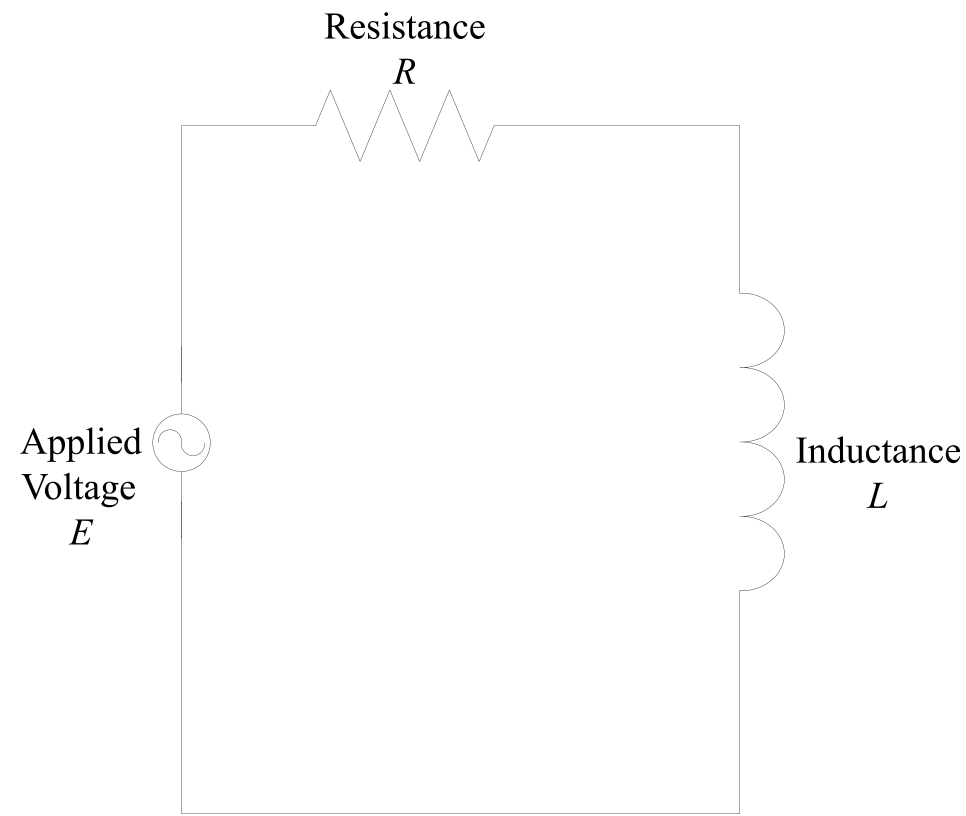
\includegraphics[ width=2.8686in, height=2.4275in,]{L4SZ283O}
}


 
\clearpage
\section{Answers}
\textbf{Exercises 7.3} 
\columnsep=30pt
\begin{multicols}{2}

1(a) $\;y =e^{t} +t^{2} +1$ 

(b) $\;y =\frac{1}{2} \left (\sin  2 x -\cos  2 x +1\right )$ 

(c) $\;y =\ln  \left \vert t\right \vert  -\frac{t^{2}}{2} +1$ 

(d) $\;P = -\frac{2}{x} +\ln  \left \vert x\right \vert  +4$ 

4. $\;y = -\frac{1}{2} x \cos  x$ 

5(a) $\;v =9.8 t\text{\quad \quad }$(b) $\;v =9.8 t +100$ 

6(a) $\;\omega  =\omega _{0} -\frac{N}{I} t\text{\quad \quad }$(b) $\;47.1 \mbox{s}$ 

\textbf{Exercises 7.4} 

1(a)  $y^{2} =x^{2} +16\text{\quad \quad }$(b) $\;v =t^{2} +1$ 

(c)  $y =2 e^{ -x} +3\text{\quad \quad }$(d)  $y =\frac{3}{2} x$ 

(e)  $i =-(9e)^{ -t} +1\text{\quad \quad }$(f)  $y =x^2+2$ 

2(b)  $5 \times 10^{10}\,$years 

3(a)  $v =50 -50 e^{ -0.2 t}\text{\quad \quad }$(b)  $3.47 \mbox{s}$ 

4(a)  $\theta  =4 +18 e^{ -k t}\text{\quad \quad }k =0.011778303$ 

(b)  $127.6989838 \approx 128\min $ (3sf) 

5(b)  $Q =100 -90 e^{ -0.1 t}\text{\quad \quad }$(c)  $66.9 \mbox{g}$ 

(e)  $Q \rightarrow 100 \mbox{g}$ 

6(c)  $142.165794 \approx 142 \mbox{min}$ (3sf) 

7.  $\rho  =\left (8\frac{1}{3} t +250\right )^{ -1}$ 

8.  $i =\frac{E}{R} \left (1 -e^{\frac{R}{L} t}\right )$ 
\end{multicols}
